% $Id$
\documentclass[11pt]{article}

% DEFAULT PACKAGE SETUP

\usepackage{setspace,graphicx,epstopdf,amsmath,amsfonts,amssymb,amsthm,versionPO}
\usepackage{marginnote,datetime,enumitem,subfigure,rotating,fancyvrb}
\usepackage{hyperref,float}
\usepackage[longnamesfirst]{natbib}
\usdate

% These next lines allow including or excluding different versions of text
% using versionPO.sty

\excludeversion{notes}		% Include notes?
\includeversion{links}          % Turn hyperlinks on?

% Turn off hyperlinking if links is excluded
\iflinks{}{\hypersetup{draft=true}}

% Notes options
\ifnotes{%
\usepackage[margin=1in,paperwidth=10in,right=2.5in]{geometry}%
\usepackage[textwidth=1.4in,shadow,colorinlistoftodos]{todonotes}%
}{%
\usepackage[margin=1in]{geometry}%
\usepackage[disable]{todonotes}%
}

% Allow todonotes inside footnotes without blowing up LaTeX
% Next command works but now notes can overlap. Instead, we'll define 
% a special footnote note command that performs this redefinition.
%\renewcommand{\marginpar}{\marginnote}%

% Save original definition of \marginpar
\let\oldmarginpar\marginpar

% Workaround for todonotes problem with natbib (To Do list title comes out wrong)
\makeatletter\let\chapter\@undefined\makeatother % Undefine \chapter for todonotes

% Define note commands
\newcommand{\smalltodo}[2][] {\todo[caption={#2}, size=\scriptsize, fancyline, #1] {\begin{spacing}{.5}#2\end{spacing}}}
\newcommand{\rhs}[2][]{\smalltodo[color=green!30,#1]{{\bf RS:} #2}}
\newcommand{\rhsnolist}[2][]{\smalltodo[nolist,color=green!30,#1]{{\bf RS:} #2}}
\newcommand{\rhsfn}[2][]{%  To be used in footnotes (and in floats)
\renewcommand{\marginpar}{\marginnote}%
\smalltodo[color=green!30,#1]{{\bf RS:} #2}%
\renewcommand{\marginpar}{\oldmarginpar}}
%\newcommand{\textnote}[1]{\ifnotes{{\noindent\color{red}#1}}{}}
\newcommand{\textnote}[1]{\ifnotes{{\colorbox{yellow}{{\color{red}#1}}}}{}}

% Command to start a new page, starting on odd-numbered page if twoside option 
% is selected above
\newcommand{\clearRHS}{\clearpage\thispagestyle{empty}\cleardoublepage\thispagestyle{plain}}

% Number paragraphs and subparagraphs and include them in TOC
\setcounter{tocdepth}{2}

% JF-specific includes:

\usepackage{indentfirst} % Indent first sentence of a new section.
\usepackage{endnotes}    % Use endnotes instead of footnotes
\usepackage{jf}          % JF-specific formatting of sections, etc.
\usepackage[labelfont=bf,labelsep=period]{caption}   % Format figure captions
\captionsetup[table]{labelsep=none}

% Define theorem-like commands and a few random function names.
\newtheorem{condition}{CONDITION}
\newtheorem{corollary}{COROLLARY}
\newtheorem{proposition}{PROPOSITION}
\newtheorem{obs}{OBSERVATION}
\newcommand{\argmax}{\mathop{\rm arg\,max}}
\newcommand{\sign}{\mathop{\rm sign}}
\newcommand{\defeq}{\stackrel{\rm def}{=}}

\begin{document}

\setlist{noitemsep}  % Reduce space between list items (itemize, enumerate, etc.)
\onehalfspacing      % Use 1.5 spacing
% Use endnotes instead of footnotes - redefine \footnote command
\renewcommand{\footnote}{\endnote}  % Endnotes instead of footnotes

\author{Jeramia Poland \thanks{\rm Indian School of Business, email \href{mailto:jeramia_poland@isb.edu}{jeramia\_poland@isb.edu}. Acknowledgments \ldots}}

\title{\Large \bf Average Variance Portfolio Management}

\date{}              % No date for final submission

% Create title page with no page number

\maketitle
\thispagestyle{empty}

\bigskip

\centerline{\bf ABSTRACT}

\begin{doublespace}  % Double-space the abstract and don't indent it
  \noindent There's nothing very interesting here, but the format (achieved using the file \texttt{jf.sty}) makes it suitable for publication in the \emph{Journal of Finance} even if the content doesn't. Here's a nice, informative, double-spaced abstract.
\end{doublespace}

\medskip

\noindent JEL classification: XXX, YYY.

\clearpage

\noindent %Discussions on investment risk and the pursuit of maximum return took place over telegraph lines nearly a century before Markowitz brought formality to the notion of risk, portfolio construction and optimization in the 1950s.\footnote{Invented by Edward A. Calahan, an employee of the American Telegraph Company in 1867 and in wide spread use starting in the 1870s, the stock ticker provided the first reliable means of conveying up to the minute stock prices over a long distances and market participants have been discusing the relationship between returns, risk, and portfolios for at least as long.\citep{rutterford_financial_2016}} %The fundamental principal that there is a "risk-premium" such that more risky investment must generate greater returns to attack capital existed from the begining. While the fundamental idea that higher risk required higher return came before, Markowitz brought formality to the notion of risk, portfolio construction and optimization in the 1950s with modern portfolio theory and mean-variance analysis. 
%Modern portfolio theory states that portfolios with higher variance need to generate higher mean returns to attract rational investors.\citep{markowitz_portfolio_1952} However, several challenges have appeared to this foundational mean-variance claim. One of the most basic is commonly referred to as the ”low-risk” or ”low-volatility” anomaly. \citet{haugen_1972} found there was little to no evidence for a "risk-premium" for increased portfolio volatility. 
While Warren Buffet may not be an enthusiastic supporter of taking leverage to invest\footnote{"When leverage works, it magnifies your gains. Your spouse thinks you're clever, and your neighbors get envious,...but leverage is addictive. Once having profited from its wonders, very few people retreat to more conservative practices. And as we all learned in third grade — and some relearned in 2008 — any series of positive numbers, however impressive the numbers may be, evaporates when multiplied by a single zero. History tells us that leverage all too often produces zeroes, even when it is employed by very smart people." \citep{noauthor_warren_nodate}}, 
%low volatility portfolios with unusually high expected returns present an opportunity for leveraged investing. 
even at fixed levels of portfolio volatility leveraged investing can be used to increase returns.
\citet{moreira_volatility-managed_2017} show across investment strategies and asset classes that merely managing leverage in a portfolio by that portfolio's volatility produces greater expected returns and performance ratios. As \citet{rutterford_financial_2016} document, the discussion of the risk-return tradeoff is at least a centurty old
%\footnote{Invented by Edward A. Calahan, an employee of the American Telegraph Company in 1867 and in wide spread use starting in the 1870s, the stock ticker provided the first reliable means of conveying up to the minute stock prices over a long distances and market participants have been discusing the relationship between returns, risk, and portfolios for at least as long.\citep{rutterford_financial_2016}} 
and central to modern financial theory, however \citet{moreira_volatility-managed_2017} demonstrate that managing investment in the market portfolio by the inverse of the prior period volatility generates greater returns and better performance ratios. Unfortunately, the volatility managed portfolio requires extreme levels of leverage. I show that managing investment in the market portfolio by the inverse of the average variance of individual daily asset returns is not only a better performer, but cheaper and more practically implementable. These improvements arise because returns to the average variance managed portfolio depend on the level of average pairwise correlation between individual asset daily returns which exposes a  systemic risk pricing dynamic which is obscured by the use of total market volatility.
 
%These results seem to challenge the mean-variance notion of investment risk premium fundamentally. 
%The notion of a risk-return tradeoff is at least a centurty old\footnote{Invented by Edward A. Calahan, an employee of the American Telegraph Company in 1867 and in wide spread use starting in the 1870s, the stock ticker provided the first reliable means of conveying up to the minute stock prices over a long distances and market participants have been discusing the relationship between returns, risk, and portfolios for at least as long.\citep{rutterford_financial_2016}} and central to modern financial theory, so naturally, I address the problem of volatility management generating excess returns by making it worse. Thankfully, this worse problem exposes evidence consistent with the explanation of low-risk anomalies which claims that investors are constrained from taking the leverage necessary in the low-risk portfolios and inconsistent with the story that investors prefer the high-risk portfolios because they enjoy lottery-like investments.
Since the early identification of a low-risk anomaly, the absence of a need to take on more risk for higher returns as in \citet{haugen_1972}, a large number of researchers have sought to identify a positive relationship between return variance and expected returns. \citet{CAMPBELL1987373}, \cite{FRENCH19873}, \citet{glosten_1993} and many, many others have found insufficient evidence identifying a positive relationship between return variance and future returns. Some investors seek to exploit aspects of this disconnection through risk management and risk-parity funds. As of 2016, at least \$150 and as much as \$400 billion sat in these funds.\citep{steward_truly_2010,cao_risk_2016} The \citet{moreira_volatility-managed_2017} results even hold for positions which already seek to exploit the low-risk anomaly like the "betting-against-beta" strategy of \citet{frazzini_betting_2014}. Additionally, other researchers have applied similar variance or volatility management to specific assets or trading styles.\footnote{See, for example, \citet{barroso_momentum_2015} and \citet{kim_time_2016} for discussions of volatility managment of the momentum portfolio.} The generation of higher expected returns without a commensurate increase in portfolio volatility implies that the representative investor, holding the market, requires less equity premium in time of high volatility. %should time asset volatility. %and appears to demand less return when it is higher. meaning the investor’s risk appetite must be higher in periods like recession and market downturns when its expected to be lower. 
In short, it seems risk does not equal reward. %However, as with pigs, some volatility is "more equal" than other volatility.\footnote{\citep{orwell1946animal}}
However, the central premiss of modern portfolio theory is that systemic risk is rewarded as investors are not able to aviod it and not all portfolio variance is systemic.

While the total variance of stock market returns (SV) is a function of both the variance of individual asset returns and the covariance between assets in the market, \citet{pollet_average_2010} show that the average pair-wise correlation of portfolio assets is the component of portfolio volatility most related to systemic changes in the economy and is the risk component compensated with higher returns. By managing the market portfolio by the other comoponent of total volatility, the average variance of the individual asset returns (AV), I generate higher average annualized monthly returns and significantly better Sharpe, Sortino, and Kappa ratios. In addition to identifying a better strategy for investors, decoupling AV from the SV sheds light on the risk-return trade-off dynamics of the market and allows leveraging investment into times when higher volatility will be compensated and pulling out when it will not.   %I then extend this by calculating the time series monthly. As expected, AV is strongly related to next period market variance and unrelated, at best insignificantly negatively, related to next period excess log returns. %As such both average variance and volatility managed portfolios represent a realization of a practical limitation of the free borrowing assumption of modern portfolio theory and not a fundamental problem with the concept of the risk-premium.
%Decoupling the idosyncratic variance of individual returns from the variance of the market portfolio returns also sheds light on the risk-return trade-off dynamics following risk shocks. ONE MORE SENTENCE HERE (transmission of shock to AC?)

%Building on this work, I use the decomposition of portfolio risk and demonstrate that even greater performance can be had by managing equity investment by the average variance of the portfolio assets rather than just the variance of the portfolio itself and in doing so I shed light on a possible explaination of the low-risk anomaly while finding evidence against another.

%Since the identification of a low-risk anomaly, or the absence of a required trade of more risk for higher returns, a large number of researchers have sought to identify a positive relationship between return variance and expected returns. \citet{CAMPBELL1987373}, \cite{FRENCH19873}, \citet{glosten_1993} and many, many others have found insufficient evidence identifying a positive relationship between return variance and future returns. On the other hand, \citet{moreira_volatility-managed_2017} demonstrate that volatility managed portfolios which decrease leverage when volatility is high produce large alphas, increase Sharpe ratios, and produce substantial utility gains for mean-variance investors. These results hold across investment styles, e.g., value or momentum, and in different asset classes, e.g., equities and currency portfolios. The results even hold for positions which already seek to exploit the low-risk anomaly like the "betting-against-beta" strategy of \citet{frazzini_betting_2014}. Additionally, other researchers have applied similar variance or volatility management to specific assets or trading styles.\footnote{See, for example, \citet{barroso_momentum_2015} and \citet{kim_time_2016} for discussions of volatility managment of the momentum portfolio.} As of 2016, at least \$150 and as much as \$400 billion sat in risk-parity funds attempting to exploit this disconnect between risk and reward.\citep{steward_truly_2010,cao_risk_2016} The generation of higher expected returns without a commensurate increase in portfolio volatility implies that a representative investor should time asset volatility, demanding less return when its higher meaning the investor’s risk appetite must be higher in periods like recession and market downturns when its expected to be lower. In short, it seems risk does not equal reward. However, as with pigs, some volatility is "more equal" than other volatility.\footnote{\citep{orwell1946animal}}

%\citet{pollet_average_2010} decompose market variance into the average correlation between pairs of assets and the average variance of the individual assets. This decomposition yields a series strongly related to both future volatility and higher returns, the average correlation of market assets series, and a one strongly related to future volatility but unrelated to returns, market asset average variance. Scaling investment in the market portfolio by the inverse of the previous period average variance should then improve return performance over and above managing investment the previous market variance since it avoids, somewhat, decreasing investment when the average correlation is high and its expected compensation. Average variance is also a better candidate for portfolio management because it has a better chance to pick up economic information sooner as individual assets respond to information about their own risk and expected returns with public disclosure while changes in aggregate materialize as data across assets are combined.\citep{campbell1997econometrics,campbell_have_2001} 

%Prior literature on the low-risk anomaly proposes two explainations. Either investors are leverage constrained and are unable to form the positions which generate the abnormal returns or investors have a preference for the extreme right tail, "lottery", returns which are not possible when employing risk managed strategies. \citet{asness_betting_2018} take a related approach to decomposing the betting-against-beta strategy of \citet{frazzini_betting_2014} into betting-against-correlation, BAC, and betting-against-variance factors, BAV, finding the BAC factor has a significant Fama-French five factor alpha but unrelated to behavior explainations of the low-risk anomally.\citep{fama_dissecting_2016} From the decomposition of daily market returns I find similar results about the more general low-risk strategy of volatility management. Management by either market variance or average asset variance actually increases the lottery-like returns of the market portfolio. Both strategies increase the Rachev ratios of the returns.

%Using daily market returns from the Center for Research in Securities Prices, I follow \citet{pollet_average_2010} generating quarterly time series of stock market variance, SV, average correlation, AC, and average variance, AV. I then extend this by calculating the time series monthly. As expected, AV is strongly related to next period market variance and unrelated, at best insignificantly negatively, related to next period excess log returns. 
%As is standard, excess log returns are the difference between the log of one plus the CRSP market return and the log of one plus the risk free return. The monthly risk free return is the return on the one month treasury bill while the quarterly risk free rate is the return on the three month treasury bill, each series is collected from the St. Louis Federal Reserve Economic Data (FRED) website. 

AV is substantially better than SV as a leverage management signal. Targeting the volatility of the buy and hold market portfolio return, as in \citet{moreira_volatility-managed_2017}, an investor without borrowing constraints earns an annualized average monthly return of 9.7\% from the AV managed portfolio. This return is a statistically significant increase of more than 1\% over the SV managed portfolio; the difference in annualized average monthly returns grows to more than 2\% when practical leverage constraints are applied. With unconstrained borrowing, the AV managed portfolio has significantly better performance ratios like the symmetric Sharpe ratio, .52, and more asymmetric risk-return measures, e.g., Kappa$_{3}$ and Kappa$_{4}$ at .15 and .11 respectively. The advantage of managing with AV grows with risk aversion. The most risk-averse, $\gamma$ = 5, constrained investor sees a certainty equivalent return (CER) gain of more than 2\% annualized; this return represents a 27.4\% increase in utility nearly as substantial as the utility gains seen in return timing strategies. \citep{campbell1997econometrics} Targeting the volatility of the buy and hold return requires seeing into the future and knowing the buy and hold return volatility. However, this look-ahead does not affect performance ratios like the Sharpe ratio, moreover the significantly better performance of AV is robust to other choices of target volatility. 
%The asset allocation gains are not all perfect, however, and the lower Rachev ratio performance of AV hints at a possible explanation for the low-risk anomaly seen in volatility and average variance management. 

The AV and SV portfolio management strategies each generate a weight in the market portfolio as a function of the daily returns of the market the prior month. Some of the investments demanded by the AV mangaged portfolio maybe difficult to achieve, however the investments needed to make the SV management strategy work are simply problematic. The SV managed portfolio takes far more extreme leverage far more often. In addition to higher average monthly borrowing costs, 15.107 vs 11.411 basis points, the SV managed portfolio has higher turnover. The AV managed portfolio generates lower transactions costs with a break even transaction cost more than 2.5 times higher than the SV managed portfolio. This makes the AV managed portfolio cheaper for the investor in both borrowing and transaction costs while generating higher returns. The AV managed portfolio is also cheaper to insure. Drawdowns are shallower and shorter for the AV managed portfiolio at 9\% vs 11.2\% and 10.5 vs 15 months on average. The drawdown profiles for the AV and SV managed portfolios also reveal that the AV managed portfolio benefits fund managers in addition to fund investors. The SV managed portfolio exposes a fund manager to twice the risk of a drawdown sever enough to threaten their job, or possibly shutter the fund, and would be nearly 91.7\% more expensive to insure. 

The identification of a better portfolio management signal is valuable, certainly to investors and fund manageers. However, a more significant contribution to our understanding of the market can be made if the reason that AV outperforms SV can be discovered. This requires examining the relationship of AV to future SV, AV, AC and returns.

Using daily market returns from the Center for Research in Securities Prices (CRSP), I extend \citet{pollet_average_2010} generating monthly time series of stock market variance, SV, average correlation, AC, and average variance, AV. From June 1962 to the end of 2016, encompassing the sample of  \citet{pollet_average_2010}, AV is a significant in-sample predictor of higher SV, AV, AC, and lower log excess market returns at the monthly frequency. A one standard deviation increase in annualized AV, from .77 to 1.62, is related to an increase in next month’s annualized SV of .545 of a standard deviation or a .22 increase. This makes next months SV more than double the mean. AV remains a significant predictor or next month's SV even when this month's SV is included. A one standard deviation increase in AV also anticipates a .13 standard deviation, .58 percentage point, lower log excess return. This makes the following month's expected return negative. When both AV and SV are used to predict next month's return, AV is significant but SV is not. %These support results at the quarterly frequency in \citet{pollet_average_2010}. 
However, over the full, 1926 to 2016, AV is a signficant predictor of higher SV, SV, AC, but not log excess market returns.%, as shown in table \ref{tab:tab_in_sample_full}. 
This evidence explains the performance of AV as a leverage management signal. Scaling investment in the market by the inverse of AV in the current month will pull funds out when the following month will have high SV without sacrificing higher expected returns. It may, in fact, avoid negative returns. These results support the intuition from the work on volatility management in \citet{moreira_volatility-managed_2017} and portfolio AV and AC in \citet{pollet_average_2010} but in-sample regression use all available information and do not necessarily identify tradeable strategies.\citep{Welch2008}
%This relationship not only holds both in and out of sample but in both National Bureau of Economic Research (NBER) defined business cycle contractions and expansions. Out of sample forecast accuracy and encompassing tests show that AV is a superior predictor of both SV and log excess returns next period.

Investors can only make decisions using the limited information available to them at a given time. For example in June of 2007 investors and investment models could only use historical information up to that month; the effects of November 2008 on the regression coefficients cannot not affect the predictions for July 2007. \citet{moreira_volatility-managed_2017} demonstrate that market volatility is an effective market portfolio management technique across the CRSP data set from 1926 to 2015. To explain why AV is a better real-time market portfolio leverage signal, I run expanding window out-of-sample regressions using AV on SV, AV, AC, and log excess returns. From June 1926 to December 2016 and using the predictions from SV as a benchmark, AV is a significantly better forecaster of next month’s AV, AC and SV. It generates better \citet{Diebold1995} test statistics, significantly lower mean squared forecast errors judging by the MSE-F statistic from \citet{mccracken_asymptotics_2007} and the emcompassing test of \citet{harvey_tests_1998} show that AV contains all of the forecasting information in SV. As with the in-sample results, AV serves investors at least as well as SV and likely better in avoiding risk without giving up return. Out-of-sample testing always raises questions about model specification, recursive expansion versus rolling window parameter estimation, choices of the training period and prediction window and the influence of specific periods. Using the techniques in \citet{rossi_out--sample_2012}, the \citet{Diebold1995} and \citet{harvey_tests_1998} measures can be calculated robust to concerns on window selection for either an expanding or rolling specification.
% robust statistics I show that the superior performance of AV, against either the running historical mean or the current time period SV in either a rolling or expanding regression specification regardless of window choice.
The \citet{rossi_out--sample_2012}  robust statistics show that AV is a significantly better predictor than SV robust to the choice of window or regression specification. %Thus, I expect managing leverage in the market portfolio by AV will produce substantially better return performance as compared to management by SV.
AV is a better leverage timing portfolio management signal than SV because is scales investment by future risk without giving up future return.

%The robust performance of AV translates into significant asset allocation gains. A strategy which weights investment in the market portfolio produces average annualized log excess returns of 7.8\% quarterly and 8.7\% monthly. The AV strategy produces quarterly and monthly Sharpe ratios, .48 and .59, each statistically significantly greater than those of the SV, volatility, management strategy. Additionally, AV generates higher values in more asymetric risk-return measures like the Sortino, Kappa, and upside potential ratios. Asset allocation performance is not all perfect, however, and the lower performance of AV in terms of Rachev ratio hints at possible explaination for the low-risk anomaly seen in volatility and average variance management. 
%As promised by the out-of-sample results, AV is substantially better than SV as a leverage management signal. Targeting the volatility of the buy and hold market portfolio return, as in \citet{moreira_volatility-managed_2017}, an investor without borrowing constraints earns an annualized average monthly return of 9.7\% from the average variance managed portfolio. This return is a statistically significant increase of more than 1\% over the SV managed portfolio; the difference in annualized average monthly returns grows to more than 2\% when practical leverage constraints are applied. With unconstrained borrowing, the AV managed portfolio has significantly better performance ratios like the symmetric Sharpe ratio, .52, and more asymmetric risk-return measures, e.g., Kappa 3 and Kappa 4 at .15 and .11 respectively. The advantage of managing with AV grows with risk aversion. The most risk-averse, $\gamma$ = 5, constrained investor sees a certainty equivalent return (CER) gain of more than 2\% annualized; this return represents a 27.4\% increase in utility nearly as substantial as the utility gains seen in return timing strategies. \citep{campbell1997econometrics} Targeting the volatility of the buy and hold return requires seeing into the future and knowing the buy and hold return volatility. However, this look-ahead does not affect performance ratios like the Sharpe ratio, moreover the significantly better performance of AV is robust to other choices of target volatility. 
%%The asset allocation gains are not all perfect, however, and the lower Rachev ratio performance of AV hints at a possible explanation for the low-risk anomaly seen in volatility and average variance management. 
%
%The AV and SV portfolio management strategies each generate a weight in the market portfolio as a function of the daily returns of the market the prior month. Some of the investments demanded by the AV mangaged portfolio maybe difficult to achieve, however the investments needed to make the SV management strategy work are simply problematic. The SV managed portfolio takes far more extreme leverage far more often. In addition to higher average monthly borrowing costs, 15.107 vs 11.411 basis points, the SV managed portfolio has higher turnover. The AV managed portfolio generates lower transactions costs with a break even transaction cost more than 2.5 times higher than the SV managed portfolio. This makes the AV managed portfolio cheaper for the investor in both borrowing and transaction costs while generating higher returns. The AV managed portfolio is also cheaper to insure. Drawdowns are shallower and shorter for the AV managed portfiolio at 9\% vs 11.2\% and 10.5 vs 15 months on average. The drawdown profiles for the AV and SV managed portfolios also reveal that the AV managed portfolio benefits fund managers in addition to fund investors. The SV managed portfolio exposes a fund manager to twice the risk of a drawdown sever enough to threaten their job, or possibly shutter the fund, and would be nearly 91.7\% more expensive to insure. 

%”There is no such thing as a free lunch,” is not only a wonderfully pervasive adage, particularly loved by economists but a provable restriction on optimization problems. \citep{wolpert_no_1997} Here, AV provides no free lunch. The improved performance measured by expected log excess returns, Sharpe, Sortino, and Kappa ratios is betrayed by worse performance in Rachev ratio. The Rachev ratio measures the right tail reward value at play relative to the left tail value at risk. In short, it measures the ratio of expected lottery rewards and losses. The volatility managed market portfolio has higher lottery winning potential for each dollar of potential lottery loss compared to the average variance managed portfolio. Both SV and AV generate better Rachev ratios than the buy and hold return. 

%%%%%%%%%%%%%%%%%%%%%%%%%%%%%%

%Prior literature on low-risk strategies, primarily cross-sectional, proposes two explanations. Either investors are leverage constrained and unable to form the positions which generate the abnormal returns or investors have a preference for the extreme right tail, ”lottery,” returns which are not possible when employing risk-managed strategies. 
%%As AV and SV managed portfolios have better Rachev ratios than the buy and hold strategy, it would seem they are better lotteries to play. 
%\citet{asness_betting_2018} take a related approach to decomposing the betting-against-beta strategy of \citet{frazzini_betting_2014} into betting-against-correlation, BAC, and betting-against-variance factors, BAV, finding the BAC factor has a significant Fama-French five-factor alpha but unrelated to behavior explanations of the low-risk anomaly. \citep{fama_dissecting_2016} From the decomposition of daily market returns, I find similar results about the more general low-risk strategy of volatility management. However, the lottery preference explaination, in this context, requires that the buy and hold market portfolio exhibit more lottery-like features than either AV or SV managed portfolios to compensate for the lost returns. Management by either market variance or average asset variance actually increases the lottery-like returns of the market portfolio. Each portfolio has larger maximum daily returns statistics, proxies used for the lottery attractiveness of an investment, than the buy and hold market. Both strategies increase the Rachev ratios of the returns. The numerator of the Rachev ratio is the expected value of extreme gains making this change is inconsistent with the notion that the lower market returns are the result of a behavioral preference for market's lottery. \citep{barberis_stocks_2008,brunnermeier_optimal_2007} Further, as \citet{barberis_stocks_2008} show that lottery preferences lead to mispricing which cannot be arbitraged away under resonable circumstances lowering the equilibrium market return. This flattens the capital market line, CML, and decreases rather than increases the seperation in market and managed returns. This effect shows up significantly in regressions testing the slop and intercept of the CML using maximum daily return statistics and gaming industry market capitalization as proxies for high lottery preferences. These CML tests come from \citet{jylha_margin_2018} who shows that lending constraints flatten the CML using margin equity requirement changes. This was first put forward by \citet{black1972capital} and appears in \citet{frazzini_betting_2014}. Again, tigher borrowing conditions flatten the CML and the returns for all market leverage portfolios are closer not further apart. I confirm the \citet{jylha_margin_2018} results using additional proxies for lending constraints like financial intermediary leverage, callable loan interest rates and margin borrowing levels. 
%
%Investors appear to be over investing in times of high market volatility and the explainations with cross-sectional bite, lottery preferences and lending constraints, do not work theorectially or empirically. Yet, what appears to a lower demand equity premium demanded for higher market volatility is actually the dynamics of the market return and the correlation of asset returns. 

%%%%%%%%%%%%%%%%%%%%%%%%%%%%%%%

%Instead, the generation of higher log excess returns by the AV, SV, and betting-against-beta strategies support the notion that the low-risk anomaly arises from leverage constraints first suggested in \citet{black1972capital}. \citet{boguth_leverage_2018} link capital constraints and the betting-against-beta strategy through mutual fund betas, and more generally \citet{malkhozov_international_2017} show that international illiquidity predicts betting-against-beta returns. Testing directly for changes in the capital market line, first shown to flatten when leverage is costly by \citet{jylha_margin_2018}, I find a significant effect of many proxies for credit constraints on the returns to AV management but no significant effect for proxies of lottery preference. Financial intermediary leverage, bank credit growth, growth in margin investing and lending rates all affect the return on the AV managed portfolio and flatten the capital market line while proxies for high investor lottery preference like market capitalization of gaming industry stocks and extreme values of market daily returns are not. The evidence is consistent with leverage constraints affecting the returns to low-risk strategies, not market-wide lottery preferences. 

%Some change in the risk-return dynamic through average variance management was anticipated given the relationship between AV and next period SV and the lack of relationship between AV and next period log excess returns. Given that idosyncratic events are reflected in individual asset volatility first we should also be able to explain the better performance of AV in terms of timing and response. Using impulse-response functions from vector auto-regression (VAR) analysis its clear that AV responds more quickly and too a larger degree to shocks than SV. A one standard deviation positive shock to AV remains significant for at least five months. Consistent with the lack of relationship show in the regression analysis the response of excess log returns to the shock in AV is negative but insignificant in the first month turning and staying positive, but in significant there after. In response, AV driven investment weight drops the first month by more than 11\%. It recovers sharply in the second month but then slowly drifts back to its initial level over the course of the next 24 months. Similar to AV, a one standard deviation shock to SV remains significant for at least five months. Excess log return reaction is also similiar to the reaction to AV but less pronounced, again consistent with the return regression results. Investment weight reaction is different however, the SV strategy sheds up to 22\% of its investment in the market before recovering. This leaves the SV strategy further out of the market during the recovery to the shock than the AV strategy which results in lost returns.

%By using the decomposition of market variance, I identify a better portfolio leverage management signal. Weighting investment leverage by the inverse of the average of individual asset variance, AV, rather than overall return variance, SV, is a new addition to the portfolio management literature letting investors capture better performance as measured by expected annualized returns. Investors also capture better investment ratios except for the Rachev ratio. The Rachev exposes the trade-off which investors must accept when managing risk by manipulating leverage conditional on average variance. The change in ratio contributes evidence against the lottery explanation of the low-risk anomaly in mean-variance analysis and supports the leverage constraints explanation. Furthur evidence shows that the returns and capital market line responds to proxies for tight lending conditions but not high lottery preference. This finding contrasts with conclusions reached in the study of cross-sectional low-risk anomalies which have been explained through the behavioral, lottery, channel.%By scarificing some potential extremely positive returns, investors using AV have access that better responds to risk shocks and participates more in the subsequent recovery. This supports prior literature which argues that individual assets should signal changes due to economic events before aggregate signals. All of this, of course, depends on the data and the construction of the individual and aggreagate signals.

Using the decomposition of market variance, I identify a better portfolio leverage management signal. Weighting investment leverage by the inverse of the average of individual asset variance, AV, rather than SV, is a new addition to the portfolio management literature letting investors capture better performance as measured by expected annualized returns, performance ratios, costs and utility gains. The returns to the AV managed portfolio serve as another example in the risk-return dynamics literature exposing the returns to correlation risk obscured when risk is measured by SV. These developments come from the formation and analysis of the AV signal. This work requires a few publically available datasets and a few considerations for the calculations at the monthly frequency. Most of the work is in the calculations required to show significance in portfolio performance and in the regression which establish the relationship of AV, risk, and future returns. 

\section{The Model} \label{sec:Model}

There's not actually a model here as it's not really a paper, but this is about where a model might go. Note that the first sentence of this section is indented (as required by the JF) using the \texttt{indentfirst} package.

\subsection{A Subsection}

Note that subsections in JF are just labeled with letters.  When referring to them in the text, you need to add the section number back, e.g., Section~\ref{sec:subsec} or~\ref{sec:subsub}. This is taken care of in \texttt{jf.sty}. Let's also add some parenthetical citations (see~\cite{Stanton:95}, \cite{CarpenterStantonWallace:12}, \cite{Campbell:03}). 

To justify adding a subsection here, from now on, we'll assume
\begin{condition}\label{cond:rates}
$0 <  \hat{\mu} < \gamma\sigma^2$.
\vspace{3mm}
\end{condition}
This condition might be useful if there was a model. 

\subsection{Another Subsection, With a Figure}
\label{sec:subsec}

Figures get put at the end, with a note marking where they should go in the text, like this:

\bigskip
\centerline{\bf [Place Figure~\ref{fig:0} about here]}
\bigskip

\subsubsection{A Subsubsection with a Proposition}
\label{sec:subsub}

Let's put a proposition here.
\begin{proposition} \label{prop:3}
If Condition~\ref{cond:rates} is satisfied,  a solution to the central
planner's problem, $V(B,D,t) \in C^2\left( {\mathbb R}_{+}^2 \times
  [0,T] \right)$, with control $a:[0,1]\times[0,T]\rightarrow [-\lambda,\lambda]$
 if  $\gamma>1$ is
\begin{equation} \label{eq:valuea}
V(B,D,t) =  - \frac{(B+D)^{1-\gamma}}{1-\gamma}   w\left(\frac{B}{B+D},t\right).
\end{equation}
\end{proposition}

\clearpage

\appendix

\section{An Appendix}
\label{sec:app1}

Here's an appendix with an equation. Note that equation numbering is quite different in appendices and that the JF wants the word ``Appendix'' to appear before the letter in the appendix title. This is all handled in \texttt{jf.sty}.
\begin{equation}
  E = mc^2.
\label{eq:eqA}
\end{equation}

\section{Another Appendix}
\label{sec:app2}

Here's another appendix with an equation.
\begin{equation}
  E = mc^2.
\end{equation}
Note that this is quite similar to Equation~\eqref{eq:eqA} in Appendix~\ref{sec:app1}.

\clearpage

% Bibliography.

\begin{doublespacing}   % Double-space the bibliography
\bibliographystyle{jf}
\bibliography{RHSbib}
\end{doublespacing}

\clearpage

% Print end notes
\renewcommand{\enotesize}{\normalsize}
\begin{doublespacing}
  \theendnotes
\end{doublespacing}

% Figures and tables, showing how to structure captions
\clearpage

\ 
\vfill
\begin{figure}[!htb]
\centerline{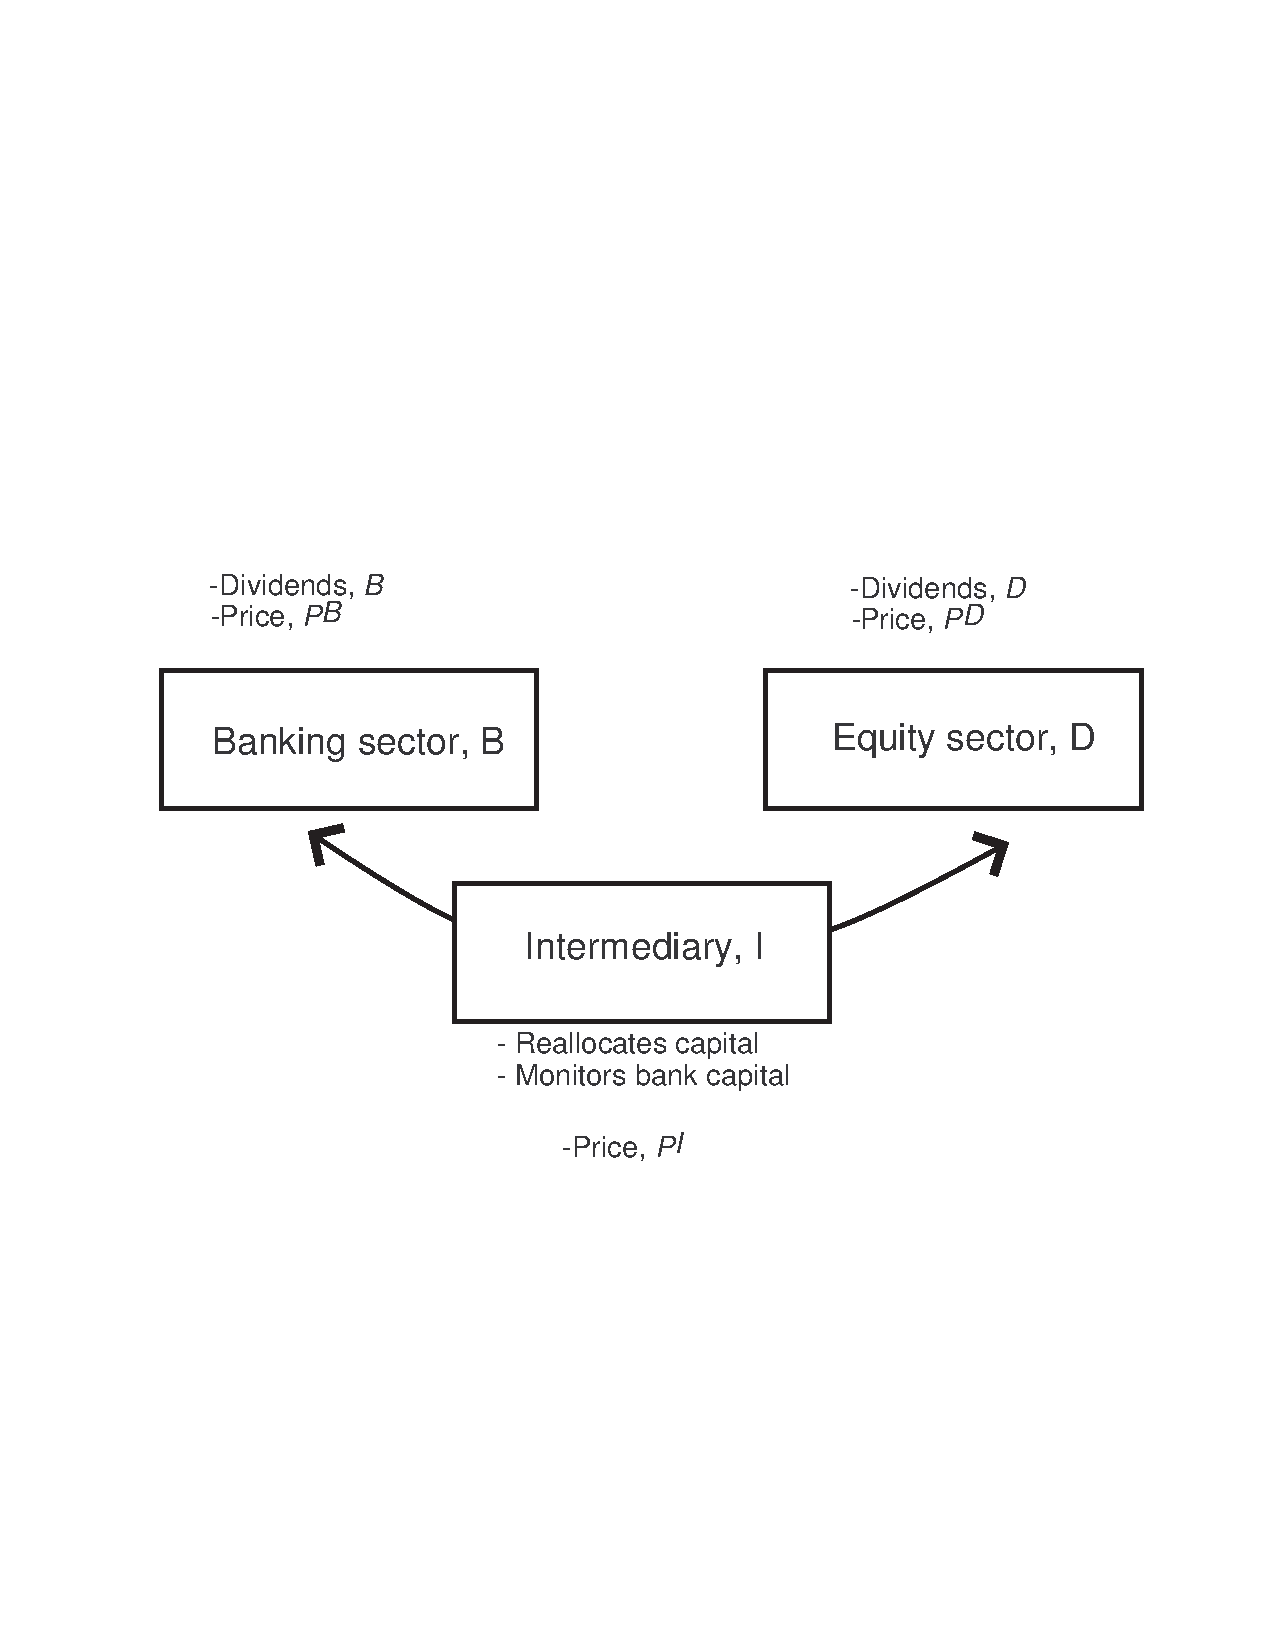
\includegraphics[width=7in]{Figure1}}
  \caption{{\bf Structure of model: capital can be invested in a bank sector and an equity sector.} An intermediary has the expertise to reallocate capital between the sectors and to monitor bank capital against bank crashes.} \label{fig:0}
\end{figure}
\vfill
\ 

\begin{table}[!htbp] 
  \centering \caption{\textbf{:Summary statistics} \newline
  	\footnotesize{Panels (a) - (c) display summary statistics for the market variance and correlation statistics, and returns. RET is the log excess return of the CRSP market portfolio. AC is the average pairwise correlation of the daily returns of the 500 largest firms in the CRSP data set over the month or quarter. AV is the average of the individual variances of daily returns for the 500 largest firms in the CRSP data set. SV is the variance of daily CRSP market returns. See section \ref{sec:Data} for details on construction.} Panel (d) displays summary statistics for international data used. The start year and month, number of months, name of the market proxy index, and the average number of assets meeting the trading and liquidity requirements for each country where the performance of AV and SV managed equity portfolios.}
  \label{tab_summary_stats}
	 \subcaption{Pollet and Wilson Sample 1963Q1:2006Q4}
	
% Table created by stargazer v.5.2 by Marek Hlavac, Harvard University. E-mail: hlavac at fas.harvard.edu
% Date and time: Tue, Mar 13, 2018 - 01:43:24  IST
\begin{table}[!htbp] \centering 
  \caption{} 
  \label{} 
\begin{tabular}{@{\extracolsep{5pt}}lccccc} 
\\[-1.8ex]\hline 
\hline \\[-1.8ex] 
Statistic & \multicolumn{1}{c}{N} & \multicolumn{1}{c}{Mean} & \multicolumn{1}{c}{St. Dev.} & \multicolumn{1}{c}{Min} & \multicolumn{1}{c}{Max} \\ 
\hline \\[-1.8ex] 
RET & 176 & 1.163 & 8.369 & $-$30.072 & 19.956 \\ 
AC & 176 & 0.230 & 0.090 & 0.034 & 0.648 \\ 
AV & 176 & 2.218 & 1.828 & 0.634 & 12.044 \\ 
SV & 176 & 0.483 & 0.616 & 0.029 & 6.397 \\ 
\hline \\[-1.8ex] 
\end{tabular} 
\end{table} 

  \subcaption{Sample 1962M6:2016M12}
    
% Table created by stargazer v.5.2 by Marek Hlavac, Harvard University. E-mail: hlavac at fas.harvard.edu
% Date and time: Tue, Mar 13, 2018 - 07:14:23  IST
\begin{table}[!htbp] \centering 
  \caption{} 
  \label{} 
\begin{tabular}{@{\extracolsep{5pt}}lccccc} 
\\[-1.8ex]\hline 
\hline \\[-1.8ex] 
Statistic & \multicolumn{1}{c}{N} & \multicolumn{1}{c}{Mean} & \multicolumn{1}{c}{St. Dev.} & \multicolumn{1}{c}{Min} & \multicolumn{1}{c}{Max} \\ 
\hline \\[-1.8ex] 
RET & 331 & 1.694 & 8.591 & $-$30.072 & 30.956 \\ 
AC & 364 & 0.282 & 0.121 & 0.034 & 0.678 \\ 
AV & 364 & 2.533 & 2.839 & 0.539 & 20.485 \\ 
SV & 364 & 0.741 & 1.258 & 0.029 & 11.378 \\ 
\hline \\[-1.8ex] 
\end{tabular} 
\end{table} 

  \subcaption{Full Sample 1926M7:2016M12}
  
% Table created by stargazer v.5.2 by Marek Hlavac, Harvard University. E-mail: hlavac at fas.harvard.edu
% Date and time: Tue, Mar 13, 2018 - 01:59:12  IST
\begin{table}[!htbp] \centering 
  \caption{} 
  \label{} 
\begin{tabular}{@{\extracolsep{5pt}}lccccc} 
\\[-1.8ex]\hline 
\hline \\[-1.8ex] 
Statistic & \multicolumn{1}{c}{N} & \multicolumn{1}{c}{Mean} & \multicolumn{1}{c}{St. Dev.} & \multicolumn{1}{c}{Min} & \multicolumn{1}{c}{Max} \\ 
\hline \\[-1.8ex] 
RET & 1,085 & 0.494 & 5.371 & $-$34.553 & 33.258 \\ 
RET3 & 1,083 & 1.482 & 9.911 & $-$55.206 & 64.968 \\ 
AC & 1,086 & 0.239 & 0.105 & 0.041 & 0.702 \\ 
AV & 1,086 & 2.432 & 2.898 & 0.502 & 33.961 \\ 
SV & 1,086 & 0.691 & 1.147 & 0.031 & 11.417 \\ 
\hline \\[-1.8ex] 
\end{tabular} 
\end{table} 

  \subcaption{Country Indices - Summary}
  \begin{tabular}{@{\extracolsep{5pt}} Hccccc} 
\\[-1.8ex]\hline 
\hline \\[-1.8ex] 
 & Country & Start & Months & Index & Avg\_Assests \\ 
\hline \\[-1.8ex] 
1 & AUS & 2000 - 5 & $212$& ASX & $200$ \\ 
2 & BRA & 1995 - 2 & $275$& iShares MSCI Brazil ETF& $60$ \\ 
3 & CHN & 2005 - 5 & $152$& CSI 300& $300$ \\ 
5 & DEU & 1993 - 11 & $290$& HDAX& $110$ \\
4 & FRA & 1993 - 9 & $292$& SBF 120& $120$ \\ 
6 & IND & 2000 - 5 & $212$& Nifty 50& $50$ \\ 
7 & ITA & 2003 - 8 & $173$& FTSE MIB& $40$ \\ 
8 & JPN & 1993 - 6 & $295$& Nikkei& $255$ \\ 
9 & UK & 1993 - 6 & $295$& FTSE& $100$ \\ 
11 & USA & 1926 - 7 & $1085$ & CRSP & 500\\
10 & World & 1995 - 3 & 274 & MSCI ACWI & 1735\\
\hline \\[-1.8ex] 
\end{tabular} 
  \end{table}

\end{document}
